\section{The Galton--Watson process}
\label{sec:galton-watson}

The Galton--Watson process is the simplest setting in which independent
reproduction, extinction and conditioning can be seen together.  Let
\(\xi,\xi_{n,i}\) be independent and identically distributed random variables with
\begin{equation}
  \Prob(\xi=k)=p_k,
  \qquad k\in\Nzero,
  \qquad
  m=\E[\xi]<\infty.
\end{equation}
Starting from one founder, \(Z_0=1\), define
\begin{equation}
  Z_{n+1}=\sum_{i=1}^{Z_n}\xi_{n,i},
  \label{eq:gw-definition}
\end{equation}
where the empty sum is zero.  State \(0\) is absorbing.  Conditional expectation in
\cref{eq:gw-definition} gives
\begin{equation}
  \E[Z_{n+1}\mid Z_n]=mZ_n,
  \qquad
  \E[Z_n]=m^n.
  \label{eq:gw-mean}
\end{equation}

Let
\begin{equation}
  \phi(z)=\E[z^\xi]=\sum_{k\geq0}p_kz^k
  \label{eq:offspring-pgf}
\end{equation}
be the offspring generating function.  The branching property implies that the
generating function of \(Z_n\) is the \(n\)-fold composition
\(\phi_n=\phi\circ\cdots\circ\phi\).  In particular, if
\begin{equation}
  u_n=\Prob(Z_n=0),
\end{equation}
then
\begin{equation}
  u_{n+1}=\phi(u_n),
  \qquad u_0=0.
  \label{eq:extinction-iteration}
\end{equation}
The limiting extinction probability is the smallest fixed point of \(\phi\) in
\([0,1]\); see, for example, \cite{Harris1963,AthreyaNey1972}.

\subsection{Binary reproduction}
\label{sec:binary-gw}

The remainder of the discrete-time analysis uses the binary offspring law
\begin{equation}
  \Prob(\xi=2)=p,
  \qquad
  \Prob(\xi=0)=1-p,
  \qquad 0\leq p\leq1.
  \label{eq:binary-law}
\end{equation}
Thus
\begin{equation}
  \phi(z)=1-p+pz^2,
  \qquad
  m=2p,
  \qquad
  \E[Z_n]=(2p)^n.
  \label{eq:binary-pgf-mean}
\end{equation}
The process is subcritical, critical or supercritical according as \(2p\) is less
than, equal to or greater than one.  Typical genealogies on either side of the
threshold are shown in \cref{fig:gw-genealogies}.

\begin{figure}[htbp]
  \centering
  
\includegraphics[width=0.72\textwidth]{simpleGWvis.png}\\[4pt]
  
\includegraphics[width=0.72\textwidth]{subGWvis.png}
  \caption{Realisations of the binary Galton--Watson process, with generation
  increasing from left to right.  The upper realisation is supercritical
  \((p=0.58)\); the lower is subcritical \((p=0.47)\).  Criticality concerns the law
  of the whole tree, not the appearance of any one finite realisation.}
  \label{fig:gw-genealogies}
\end{figure}

For the binary law, \cref{eq:extinction-iteration} becomes
\begin{equation}
  u_{n+1}=1-p+pu_n^2.
  \label{eq:binary-u-recursion}
\end{equation}
It is convenient to use the survival probability
\begin{equation}
  S_n=1-u_n=\Prob(Z_n>0).
  \label{eq:Sn-definition}
\end{equation}
Substitution into \cref{eq:binary-u-recursion} gives the logistic recursion
\begin{equation}
  S_{n+1}=2pS_n-pS_n^2,
  \qquad S_0=1.
  \label{eq:Sn-recursion}
\end{equation}
The sequence \(u_n\) is non-decreasing because extinction is absorbing; hence
\(S_n\) is non-increasing and has a limit.  Any such limit is a fixed point of
\cref{eq:Sn-recursion}.  Solving
\begin{equation}
  S=2pS-pS^2
\end{equation}
gives
\begin{equation}
  S=0
  \qquad\text{or}\qquad
  S=\frac{2p-1}{p}.
  \label{eq:survival-fixed-points}
\end{equation}
The second root is inadmissible for \(p<1/2\), coalesces with zero at \(p=1/2\),
and lies in \((0,1]\) for \(p>1/2\).  It follows that
\begin{equation}
  S_\infty:=\Prob(Z_n>0\text{ for every }n)
  =
  \begin{cases}
    0, & 0\leq p\leq\tfrac12,\\[2mm]
    \dfrac{2p-1}{p}, & \tfrac12<p\leq1.
  \end{cases}
  \label{eq:ultimate-survival}
\end{equation}
The phase transition is continuous, but the stability of the zero fixed point
changes at \(p=1/2\), as \cref{fig:gw-fixed-points} makes explicit.

\begin{figure}[htbp]
\centering
\begin{subfigure}[b]{0.31\textwidth}
\centering
\begin{tikzpicture}
\begin{axis}[
  width=4.35cm,height=4.2cm,axis lines=left,
  xmin=0,xmax=1,ymin=0,ymax=1,
  xtick={0,0.5,1},ytick={0,0.5,1},
  tick label style={font=\scriptsize},
  xlabel={$S_n$},ylabel={$S_{n+1}$},
  label style={font=\scriptsize},samples=100]
  \addplot[blue,thick,domain=0:1]{0.6*x-0.3*x^2};
  \addplot[black!55,dashed,domain=0:1]{x};
  \fill[red] (axis cs:0,0) circle[radius=1.5pt];
\end{axis}
\end{tikzpicture}
\caption{\(p=0.3\)}
\end{subfigure}
\hfill
\begin{subfigure}[b]{0.31\textwidth}
\centering
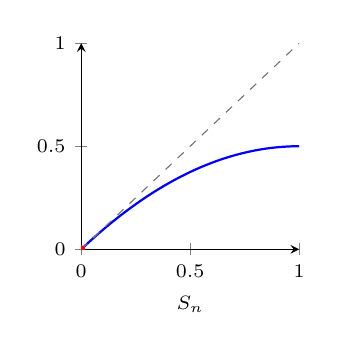
\begin{tikzpicture}
\begin{axis}[
  width=4.35cm,height=4.2cm,axis lines=left,
  xmin=0,xmax=1,ymin=0,ymax=1,
  xtick={0,0.5,1},ytick={0,0.5,1},
  tick label style={font=\scriptsize},
  xlabel={$S_n$},label style={font=\scriptsize},samples=100]
  \addplot[blue,thick,domain=0:1]{x-0.5*x^2};
  \addplot[black!55,dashed,domain=0:1]{x};
  \fill[red] (axis cs:0,0) circle[radius=1.5pt];
\end{axis}
\end{tikzpicture}
\caption{\(p=0.5\)}
\end{subfigure}
\hfill
\begin{subfigure}[b]{0.31\textwidth}
\centering
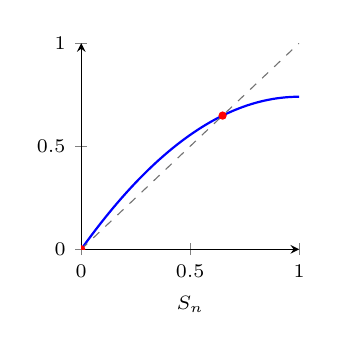
\begin{tikzpicture}
\begin{axis}[
  width=4.35cm,height=4.2cm,axis lines=left,
  xmin=0,xmax=1,ymin=0,ymax=1,
  xtick={0,0.5,1},ytick={0,0.5,1},
  tick label style={font=\scriptsize},
  xlabel={$S_n$},label style={font=\scriptsize},samples=100]
  \addplot[blue,thick,domain=0:1]{1.48*x-0.74*x^2};
  \addplot[black!55,dashed,domain=0:1]{x};
  \fill[red] (axis cs:0,0) circle[radius=1.5pt];
  \fill[red] (axis cs:0.64864865,0.64864865) circle[radius=1.5pt];
\end{axis}
\end{tikzpicture}
\caption{\(p=0.74\)}
\end{subfigure}

\medskip
\begin{tikzpicture}
\begin{axis}[
  width=8.3cm,height=5.1cm,axis lines=left,
  xmin=0,xmax=1,ymin=0,ymax=1,
  xtick={0,0.5,1},ytick={0,0.5,1},
  xlabel={$p$},ylabel={$S_\infty$},
  grid=major,grid style={dashed,gray!25},samples=140]
  \addplot[red,very thick,domain=0:0.5]{0};
  \addplot[red,very thick,domain=0.5:1]{(2*x-1)/x};
  \fill[black] (axis cs:0.5,0) circle[radius=1.5pt];
\end{axis}
\end{tikzpicture}
\caption{The survival map \(S\mapsto2pS-pS^2\) against the diagonal and the
resulting ultimate survival probability.  At criticality the map is tangent to the
diagonal at the origin.}
\label{fig:gw-fixed-points}
\end{figure}

\subsection{Critical decay and extinction time}
\label{sec:critical-gw}

At \(p=1/2\), the mean in \cref{eq:binary-pgf-mean} is one at every generation,
even though \cref{eq:ultimate-survival} says that extinction is certain.  The
resolution is a heavy tail: rare surviving trees are sufficiently large to keep the
unconditional mean fixed.  The corresponding survival asymptotic can be obtained
directly from the exact recursion, without a continuum approximation.

\begin{proposition}[Critical survival probability]
\label{prop:critical-survival}
For the critical binary process,
\begin{equation}
  S_n\sim\frac{2}{n}
  \qquad(n\to\infty).
  \label{eq:critical-Sn}
\end{equation}
\end{proposition}

\begin{proof}
At \(p=1/2\), \cref{eq:Sn-recursion} reads
\begin{equation}
  S_{n+1}=S_n-\frac12S_n^2=S_n\left(1-\frac{S_n}{2}\right).
  \label{eq:critical-recursion}
\end{equation}
Because \(S_n\downarrow0\), the reciprocal sequence tends to infinity.  Its
increments satisfy
\begin{equation}
  \frac{1}{S_{n+1}}-\frac{1}{S_n}
  =\frac{1}{2(1-S_n/2)}\longrightarrow\frac12.
  \label{eq:reciprocal-increment}
\end{equation}
The Stolz--Ces\`aro theorem, or summation of the convergent increments, now gives
\((1/S_n)/n\to1/2\), which is equivalent to \cref{eq:critical-Sn}.
\end{proof}

Let
\begin{equation}
  T=\inf\{n\geq0:Z_n=0\}
  \label{eq:extinction-time}
\end{equation}
be the extinction time.  Since \(T=\sum_{n\geq0}\ind_{\{T>n\}}\), Tonelli's theorem
gives the tail-sum identity
\begin{equation}
  \E[T]=\sum_{n=0}^{\infty}\Prob(T>n)
       =\sum_{n=0}^{\infty}S_n.
  \label{eq:mean-extinction-tail-sum}
\end{equation}
By \cref{eq:critical-Sn}, the final series has the same divergent tail as
\(2\sum_n n^{-1}\).  Thus extinction occurs almost surely but
\begin{equation}
  \E[T]=\infty.
  \label{eq:critical-infinite-lifetime}
\end{equation}
The point probabilities follow from the exact decrement in
\cref{eq:critical-recursion}:
\begin{equation}
  \Prob(T=n+1)=S_n-S_{n+1}=\frac12S_n^2
  \sim\frac{2}{n^2}.
  \label{eq:critical-T-tail}
\end{equation}

The total progeny
\begin{equation}
  \mathcal T=\sum_{n\geq0}Z_n
  \label{eq:total-progeny}
\end{equation}
has a different critical exponent.  A finite binary genealogy with \(k\) division
vertices contains \(k+1\) terminal vertices and hence \(2k+1\) individuals in all.
The number of such ordered full binary trees is the Catalan number
\(C_k=(k+1)^{-1}\binom{2k}{k}\).  Consequently,
\begin{equation}
  \Prob(\mathcal T=2k+1)=C_kp^k(1-p)^{k+1}.
  \label{eq:total-progeny-exact}
\end{equation}
At \(p=1/2\), Stirling's formula yields
\begin{equation}
  \Prob(\mathcal T=2k+1)
  \sim\frac{1}{2\sqrt{\pi}}k^{-3/2}.
  \label{eq:total-progeny-asymptotic}
\end{equation}
The \(3/2\) law therefore holds along the admissible odd values; the probability is
zero at even values.  \Cref{fig:critical-power-laws} places the survival, extinction-
time and total-progeny scalings side by side.

\begin{figure}[htbp]
  \centering
  
\includegraphics[width=0.97\textwidth]{power_law_fixed.pdf}
  \caption{Critical power laws from \(10^6\) simulated binary Galton--Watson
  realisations.  From left to right: \(S_n\sim2/n\),
  \(\Prob(T=n)\sim2/n^2\), and the \(n^{-3/2}\) total-progeny law on its odd
  support.  The first two exponents also follow directly from
  \cref{eq:critical-recursion}.}
  \label{fig:critical-power-laws}
\end{figure}

\FloatBarrier
